%!TEX root = ../thesis.tex

\chapter{Marco Metodológico}  %Title of the First Chapter
\label{capitulo3}

\ifpdf
    \graphicspath{{metodologia/Figs/Raster/}{metodologia/Figs/PDF/}{metodologia/Figs/}}
\else
    \graphicspath{{metodologia/Figs/Vector/}{metodologia/Figs/}}
\fi

A fin de mejorar la productividad en el desarrollo y la calidad del motor de juego, se hace uso de la metodología de desarrollo por prototipos. Esta  metodología se caracteriza por la construcción de un prototipo, el cual es evaluado y usado en un ciclo de retroalimentación, en donde se refinan los requisitos del software que se desarrollará \cite{mcconnell2004code}. Esta metodología permite probar la eficacia de diferentes algoritmos y la forma que debería tomar la interacción humano-máquina a través de diferentes prototipos, aspectos importantes para este proyecto, debido a que los algoritmos tradicionales para motores de juegos diseñados para lenguajes iterativos no son ideales para su uso en lenguajes funcionales.

\begin{figure}[!htbp!]
\centering
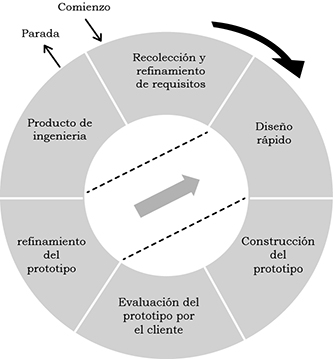
\includegraphics[width=0.5\textwidth]{metoPrototipo}
\caption[Metodología de desarrollo por prototipos]{Ciclo de desarrollo de una aplicación mediante la metodología de desarrollo por prototipos.}
\end{figure}

\section{Requerimientos del sistema}

Ya que el objetivo de este proyecto es la creación de un motor de juego, este debe, al igual que otros motores de juego, tener un motor gráfico para dibujar en pantalla, permitir a los programadores implementar la lógica de sus juegos, permitir a los artistas importar recursos al juego, un motor de física que resuelva colisiones entre objetos, entre otras características comunes antes mencionadas.

La diferencia que este proyecto debe necesariamente suplir, es funcionar en un lenguaje funcional, permitiendo a los programadores de los juegos trabajar con el mismo, y hacer el mayor uso posible de los beneficios que brinda la programación funcional para hacer que los juegos producidos sean lo más eficientes posible.

El programa final tendrá como usuario tres tipos de actores, que son los artistas, interesados principalmente en poder usar sus creaciones dentro del juego, los programadores, que implementan la lógica del juego usando el motor, y los jugadores, que si bien no interactúan directamente con el motor, lo hacen indirectamente a través de los juegos creados. Véase el diagrama de casos de uso en la \emph{Figura~\ref{fig:MCU}}.

\subsection{Requerimientos funcionales}

\begin{itemize}
  \item Generar videojuegos funcionales, el motor debe de ofrecer una interfaz mediante la cual los programadores que usen el motor puedan implementar la lógica de sus juegos y el motor debe de encargarse de enlazar los sistemas necesarios para generar un juego funcional.
  \item Administrar la entrada del videojuego, el motor debe de garantizar que la entrada generada por el jugador pueda ser correctamente procesada.
  \item Permitir la carga de recursos multimedia al juego, el motor debe de proveer facilidades para ingresar contenido de los artistas dentro del juego.
\end{itemize}

\subsection{Requerimientos no funcionales}

\begin{itemize}
  \item Administrar los recursos del dispositivo, el motor debe hacer un uso eficiente de los recursos del dispositivo para proveer una mejor experiencia de juego.
  \item Concurrencia, el motor debe de poder hacer uso de la concurrencia para ofrecer un mejor desempeño, aprovechando las ventajas de lenguaje Haskell para este fin.
\end{itemize}

\section{Limitaciones del sistema}

Ya que crear un motor de juego con todas las características que poseen los motores profesionales es una labor de gran envergadura, este proyecto limitara las funcionalidades del programa final en lo mínimo requerido para poder producir juegos funcionales.

Las capacidades mínimas elegidas para poder producir juegos son, tener un  motor gráfico, poder cargar recursos para el motor gráfico, en este caso imágenes, shaders y mallados poligonales, y finalmente el motor lógico donde el programador implementará la funcionalidad del juego. Están serán tomadas como los requerimientos  mínimos que el programa final deberá de proveer como motor de juego, y serán usados como guía para la producción de los prototipos durante el desarrollo.

\section{Arquitectura}

Los diferentes requerimientos del proyecto serán implementados en forma modular, para permitir que nuevos prototipos solo requieran la modificación de una sección del programa. Como el lenguaje de implementación \emph{Haskell} posee estándares para la construcción de paquetes y librerías \cite{wiki:WriteAHaskellProgram}, estos se utilizaran para la construcción de la herramienta.

Los videojuegos creados usaran una arquitectura en pipeline, que consiste en la transformación contínua del flujo de datos (entrada del jugador) en un resultado (gráficos del juego). Este modelo surge naturalmente en la programación funcional por su equivalencia a la composición de funciones y al flujo de trabajo encontrado en las librerías de FRP.

\section{Desarrollo}

Usando la metodología de desarrollo por prototipos, se implementará módulos que busquen satisfacer los requisitos del sistema junto con prototipos que hagan uso de estos módulos. A través de estos prototipos se decidirá la satisfacción de los requisitos y se entrará en un ciclo de corrección y ajuste.

\section{Documentación}

El presente documento servirá como el principal manual para el funcionamiento interno del programa. Para documentación que indique el uso y funcionamiento de las funciones públicas implementadas por el motor, se usara el estándar de comentarios de \emph{Haskell} para generar documentación. Usando el programa ¨stack¨ sera posible generar la documentación en html usando el comando ¨stack haddock¨ en el directorio raíz del código provisto junto a este documento.

\section{Pruebas funcionales}

Para realizar pruebas continuas en cada iteración de la contrucción de la herramienta se crearon cuatro juegos de prueba usando la misma herramienta para prevenir que algún componente se viese afectado en cualquiera de las iteraciones.

\begin{enumerate}
  \item Programa de prueba 1: juego en que cubos y esferas se mueven sobre un mapa, los objetos iguales rebotan entre sí y los diferentes se eliminan al chocar. Adicionalmente el jugador puede controlar la cámara con el ratón y teclado. Véase \emph{Figura~\ref{fig:test1}}.
  \item Programa de prueba 2: juego en que una esfera rebota sobre un plano, el jugador puede controlar la cámara con el ratón y teclado. Véase \emph{Figura~\ref{fig:test2}}.
  \item Programa de prueba 3: juego en que 200 esferas rebotan entre sí. Esta resultó la prueba más importante para medir rendimiento por la cantidad de elementos en escena. Véase \emph{Figura~\ref{fig:test3}}.
  \item Programa de prueba 4: juego en que un cono persigue a una esfera controlada por el jugador. Adicionalmente el jugador puede controlar la cámara con el ratón y teclado. Véase \emph{Figura~\ref{fig:gameia}}.
\end{enumerate}

Estos programas de prueba pueden ser compilados y ejecutados corriendo los siguientes comandos desde el directorio raíz del código provisto junto a este documento:

\begin{lstlisting}[frame=single,language=Haskell]
stack build
stack exec test1
stack exec test3
stack exec test2
stack exec gameia
\end{lstlisting}
